\section{Volatility}
Volatility is a memory analysis tool. Similar to Redline.\\
Volatility uses python2 and python3. This tool is plugin-based.
\begin{lstlisting}
volatility2 -f hiberfile.sys -O hiberfile.raw --profile=<profile> imagecopy
\end{lstlisting}
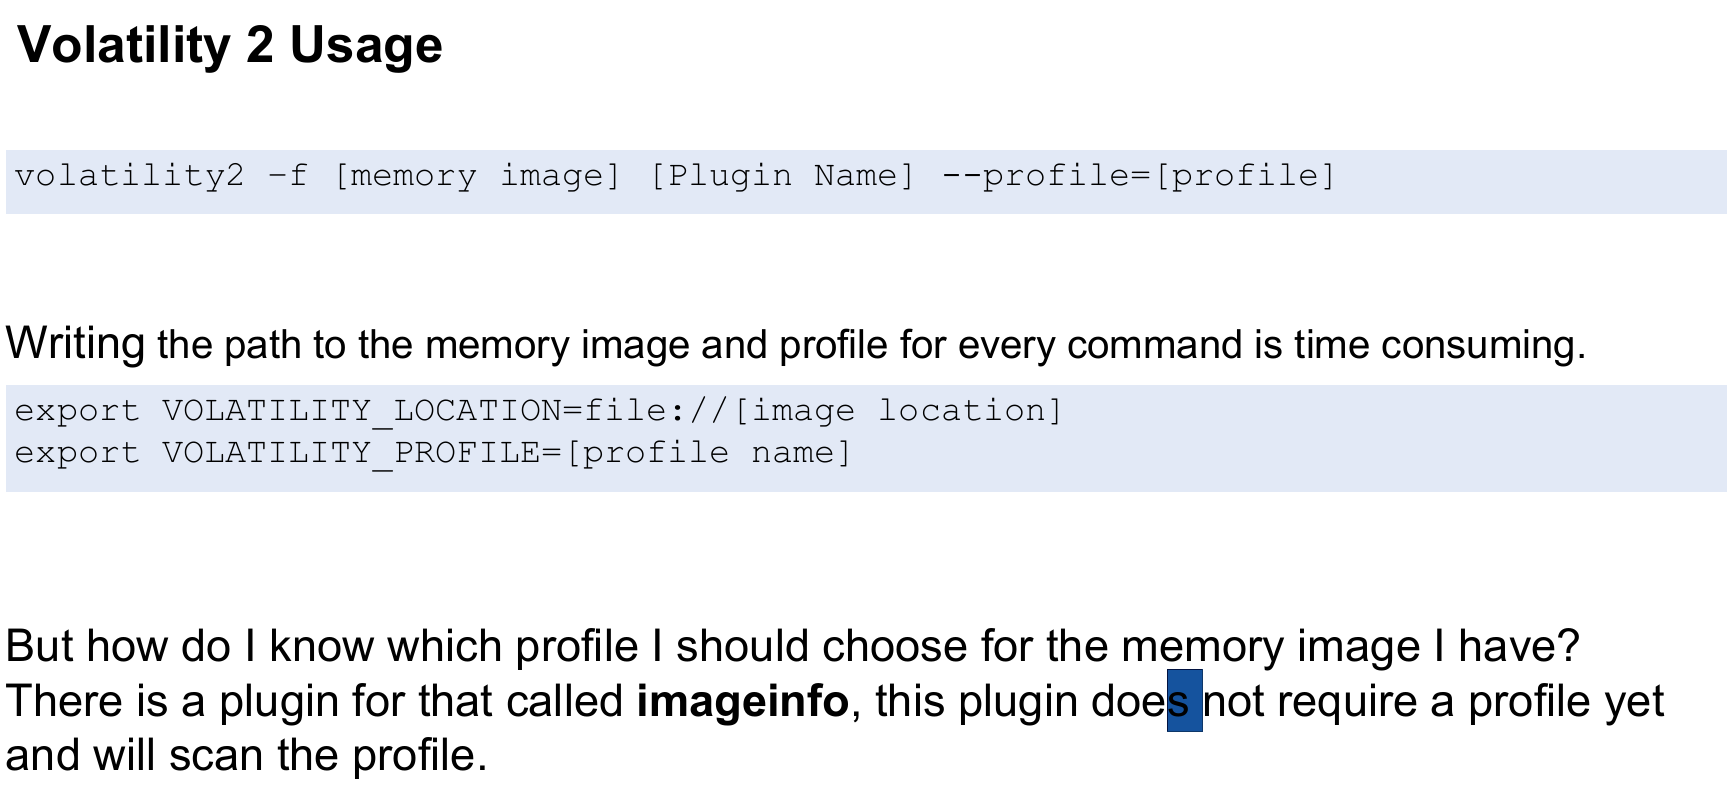
\includegraphics[width=\linewidth]{vol2.png}


\paragraph{Evidence}
\begin{itemize}
  \item Physical Memory
  \item Pagefile
  \item Crash Dumps
  \item Hibernation Files
\end{itemize}

\paragraph{Artifacts}
\begin{itemize}
  \item Processes
  \item Network connections
  \item Loaded drivers
  \item Console command history
  \item Strings in memory
  \item Credentials and keys
  \item Everything running on a computer
\end{itemize}

\subsection{Memory Acquisition}
\paragraph{Windows}
\begin{itemize}
  \item WinPMEM Rekall
  \item FTK Imager Access Data
  \item FDPro HBGary
  \item Memoryze FireEye
  \item F-Response
\end{itemize}
\textbf{Example with winpmem:}
\begin{lstlisting}
  C:\> winpmem.exe -0 dump0.raw
\end{lstlisting}

\paragraph{Linux}
\begin{itemize}
  \item AVML (Acquire Volatile Memory for Linux)
  \item LiME Linux Memory Extractor
\end{itemize}
\textbf{Example with LiME:}
\begin{lstlisting}
  #insmod /var/lib/dkms/lime-forensics/.../module/lime.ko "path=dump.raw format=raw"
\end{lstlisting}

\subsection{Usage}
Check Slides for usage.